





\textit{Uniform Resource Identifier} (URI) adalah sebuah mekanisme yang digunakan untuk mengidentifikasi \textit{resource}. URI dapat diklasifikasikan lebih lanjut sebagai lokasi, nama, atau keduanya. Sebagai lokasi, URI memiliki \textit{subset} bernama \textit{Uniform Resource Locator} (URL),  yaitu URI yang menjelaskan mekanisme utama untuk menemukan \textit{resource}. Sedangkan sebagai nama, URI memiliki \textit{subset} bernama \textit{Uniform Resource Name} (URN)~\cite{RFC2141}, yaitu URI yang berfungsi sebagai pengenal \textit{resource} yang bersifat unik secara global, persisten dan tidak bergantung pada lokasi.


\subsection{Komponen Sintaksis}
\label{subsec:0202-komponen-sintaksis}
Sintaks URI disusun sebagai urutan hierarkis dari beberapa komponen utama, yaitu \textit{scheme}, \textit{authority}, \textit{path}, \textit{query}, dan \textit{fragment}. Komponen \textit{scheme} dan \textit{path} bersifat wajib, meskipun \textit{path} dapat berupa string kosong. Apabila komponen \textit{authority} hadir, maka \textit{path} harus kosong atau diawali dengan garis miring (``/''). Sebaliknya, apabila \textit{authority} tidak hadir, maka \textit{path} tidak boleh diawali dengan dua garis miring (``//''). Sebagai ilustrasi, Gambar~\ref{fig:contoh-url} menunjukkan contoh URL yang disusun dari komponen utama yang lengkap.

\begin{figure}[H]
    \centering
    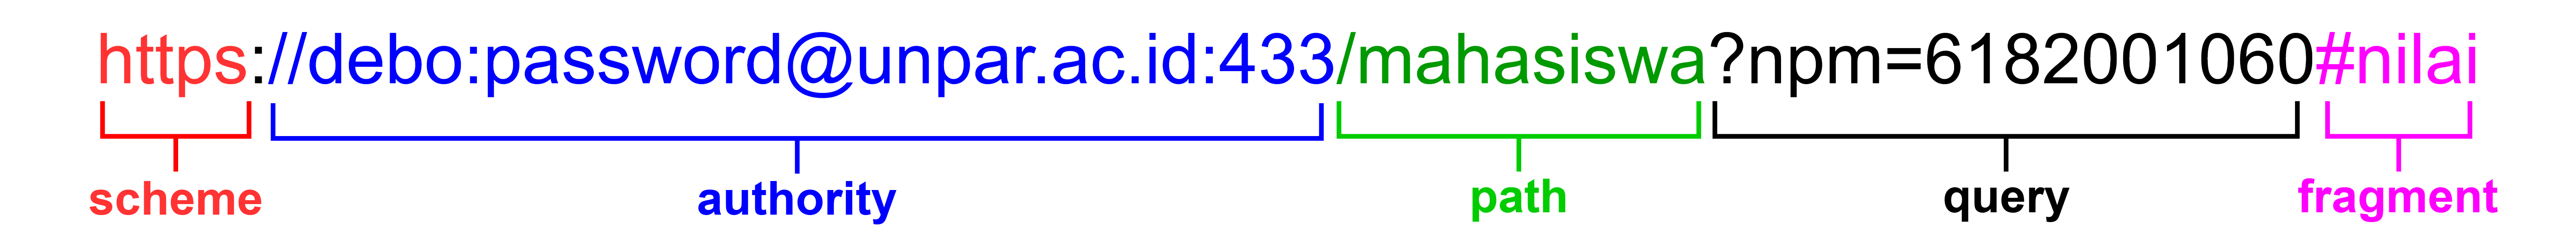
\includegraphics[width=0.90\textwidth]{Gambar/020201-contoh-url.png}
    \caption{Contoh URL}
    \label{fig:contoh-url}
\end{figure}


\begin{enumerate}
    \item \textbf{\textit{Scheme}}\\  
    Komponen ini merupakan awalan dari sebuah URI dan akan diakhiri dengan tanda titik dua (``:''). Nama dari \textit{scheme} merujuk pada suatu spesifikasi yang menetapkan bagaimana pengidentifikasi dalam \textit{scheme} tersebut ditentukan. Pada contoh URL yang diberikan pada Gambar~\ref{fig:contoh-url}, \textit{scheme} adalah \texttt{https}.
    
    \item \textbf{\textit{Authority}}\\  
    Komponen ini diawali dengan tanda ganda garis miring (``//'') dan berakhir sebebelum garis miring (``/''), tanda tanya (``?''), tanda pagar (``\#''), atau akhir dari URI. Secara umum, \textit{authority} terdiri dari:
    
    \begin{itemize}
        
        \item \textbf{\textit{User Information}}: Bagian opsional yang dapat berisi nama pengguna atau informasi lain yang terkait otorisasi, diakhiri dengan \textit{at-sign} (``@''). Pada contoh URL yang diberikan pada Gambar~\ref{fig:contoh-url}, \textit{user information} adalah \texttt{debo:password}.
        
        \item \textbf{\textit{Host}}: Menunjukkan nama host atau alamat IP yang menjadi identitas tujuan. Pada contoh URL yang diberikan pada Gambar~\ref{fig:contoh-url}, \textit{host} adalah \texttt{unpar.ac.id}.
        
        \item \textbf{\textit{Port}}: Bagian opsional berupa angka desimal setelah tanda titik dua (``:''). Jika tidak ditulis, maka port bawaan dari \textit{scheme} digunakan. Pada contoh URL yang diberikan pada Gambar~\ref{fig:contoh-url}, \textit{port} adalah \texttt{433}.
    
    \end{itemize}
    
    \item \textbf{\textit{Path}}\\  
    Bagian ini menunjukkan lokasi sumber daya dalam hierarki host. \textit{Path} selalu didefinisikan, walaupun dapat berupa string kosong. Pada contoh URL yang diberikan pada Gambar~\ref{fig:contoh-url}, \textit{path} adalah \texttt{mahasiswa}.
    
    \item \textbf{\textit{Query}}\\  
    Komponen ini berisi data non-hierarkis yang biasanya berupa pasangan \textit{key=value}. Bagian ini diawali dengan tanda tanya (``?'') dan berakhir sebelum tanda pagar (``\#'') atau akhir URI. Pada contoh URL yang diberikan pada Gambar~\ref{fig:contoh-url}, \textit{query} adalah \texttt{npm=6182001060}.
    
    \item \textbf{\textit{Fragment}}\\  
    Bagian ini memungkinkan identifikasi sekunder terhadap suatu sumber daya, misalnya bagian tertentu dari sebuah dokumen. \textit{Fragment} diawali dengan tanda pagar (``\#'') dan diakhiri dengan akhir URI. Pada contoh URL yang diberikan pada Gambar~\ref{fig:contoh-url}, \textit{fragment} adalah \texttt{nilai}.
\end{enumerate}



\subsection{Karakter}
\label{subsec:0202-karakter}

\begin{itemize}
    \item \textbf{\textit{Percent-Encoding}}
    
    \item \textbf{\textit{Reserved Characters}}
    
    \item \textbf{\textit{Unreserved Characters}}
    
\end{itemize}



\subsection{Resolusi Referensi}
\label{subsec:0202-resolusi-referensi}

\begin{enumerate}
    \item \textit{Base} URI
    \begin{enumerate}
        \item \textit{Base} URI dalam konten
        \item \textit{Base} URI dari entitas pengenkapsulasi
        \item \textit{Base} URI dari URI pengambilan
        \item Default \textit{Base} URI
    \end{enumerate}

    \item \textit{Proses Resolusi Relatif}
    \begin{enumerate}
        \item Pre-parse Base URI
        \item Transformasi Referensi
        \item Merge Path
        \item Remove Dot Segments
    \end{enumerate}

    \item \textit{Rekomposisi Komponen}
    
    \item \textit{Contoh Resolusi} (normal dan abnormal)
    
\end{enumerate}


\subsection{IRI}
\label{subsec:0202-iri}